% !TEX TS-program = XeLaTeX
% use the following command:
% all document files must be coded in UTF-8
\documentclass[spanish]{textolivre}
% build HTML with: make4ht -e build.lua -c textolivre.cfg -x -u article "fn-in,svg,pic-align"

\journalname{Texto Livre}
\thevolume{15}
%\thenumber{1} % old template
\theyear{2022}
\receiveddate{\DTMdisplaydate{2021}{06}{22}{-1}} % YYYY MM DD
\accepteddate{\DTMdisplaydate{2021}{10}{4}{-1}}
\publisheddate{\DTMdisplaydate{2021}{11}{4}{-1}}
\corrauthor{Guillermo Rodríguez-Martínez}
\articledoi{10.35699/1983-3652.2022.34828}
%\articleid{NNNN} % if the article ID is not the last 5 numbers of its DOI, provide it using \articleid{} commmand
% list of available sesscions in the journal: articles, dossier, reports, essays, reviews, interviews
\articlesessionname{articles}
\runningauthor{Rodríguez-Martínez y Arango Lozano} 
%\editorname{Leonardo Araújo} % old template
\sectioneditorname{Daniervelin Pereira}
\layouteditorname{Anna Izabella Miranda Pereira}

\title{Uso de internet y redes sociales en el marco de la contingencia Covid-19 en Colombia: análisis en población juvenil considerando su nivel socio-económico}
\othertitle{Uso da internet e redes sociais no marco da contingência Covid-19 na Colômbia: análise da população jovem considerando seu nível socioeconômico}
\othertitle{Use of internet and social networks within the framework of the Covid-19 situation in Colombia: analysis of young people considering their socio-economic level}
% if there is a third language title, add here:
%\othertitle{Artikelvorlage zur Einreichung beim Texto Livre Journal}

\author[1]{Guillermo Rodríguez-Martínez~\orcid{0000-0003-4329-5745}~\thanks{Email:~\url{guillermo.rodriguez@utadeo.edu.co}}}
\author[1]{Carlos Andrés Arango Lozano~\orcid{0000-0002-2786-3653}~\thanks{Email:~\url{carlosa.arangol@utadeo.edu.co}}}
\affil[1]{Universidad Jorge Tadeo Lozano, Bogotá, Colombia.}

\addbibresource{article.bib}
% use biber instead of bibtex
% $ biber article

% used to create dummy text for the template file
\definecolor{dark-gray}{gray}{0.35} % color used to display dummy texts
\usepackage{lipsum}
\SetLipsumParListSurrounders{\colorlet{oldcolor}{.}\color{dark-gray}}{\color{oldcolor}}

% used here only to provide the XeLaTeX and BibTeX logos
\usepackage{hologo}

% if you use multirows in a table, include the multirow package
\usepackage{multirow}

% provides sidewaysfigure environment
\usepackage{rotating}

% CUSTOM EPIGRAPH - BEGIN 
%%% https://tex.stackexchange.com/questions/193178/specific-epigraph-style
\usepackage{epigraph}
\renewcommand\textflush{flushright}
\makeatletter
\newlength\epitextskip
\pretocmd{\@epitext}{\em}{}{}
\apptocmd{\@epitext}{\em}{}{}
\patchcmd{\epigraph}{\@epitext{#1}\\}{\@epitext{#1}\\[\epitextskip]}{}{}
\makeatother
\setlength\epigraphrule{0pt}
\setlength\epitextskip{0.5ex}
\setlength\epigraphwidth{.7\textwidth}
% CUSTOM EPIGRAPH - END

% LANGUAGE - BEGIN
% ARABIC
% for languages that use special fonts, you must provide the typeface that will be used
% \setotherlanguage{arabic}
% \newfontfamily\arabicfont[Script=Arabic]{Amiri}
% \newfontfamily\arabicfontsf[Script=Arabic]{Amiri}
% \newfontfamily\arabicfonttt[Script=Arabic]{Amiri}
%
% in the article, to add arabic text use: \textlang{arabic}{ ... }
%
% RUSSIAN
% for russian text we also need to define fonts with support for Cyrillic script
% \usepackage{fontspec}
% \setotherlanguage{russian}
% \newfontfamily\cyrillicfont{Times New Roman}
% \newfontfamily\cyrillicfontsf{Times New Roman}[Script=Cyrillic]
% \newfontfamily\cyrillicfonttt{Times New Roman}[Script=Cyrillic]
%
% in the text use \begin{russian} ... \end{russian}
% LANGUAGE - END

% EMOJIS - BEGIN
% to use emoticons in your manuscript
% https://stackoverflow.com/questions/190145/how-to-insert-emoticons-in-latex/57076064
% using font Symbola, which has full support
% the font may be downloaded at:
% https://dn-works.com/ufas/
% add to preamble:
% \newfontfamily\Symbola{Symbola}
% in the text use:
% {\Symbola }
% EMOJIS - END

% LABEL REFERENCE TO DESCRIPTIVE LIST - BEGIN
% reference itens in a descriptive list using their labels instead of numbers
% insert the code below in the preambule:
%\makeatletter
%\let\orgdescriptionlabel\descriptionlabel
%\renewcommand*{\descriptionlabel}[1]{%
%  \let\orglabel\label
%  \let\label\@gobble
%  \phantomsection
%  \edef\@currentlabel{#1\unskip}%
%  \let\label\orglabel
%  \orgdescriptionlabel{#1}%
%}
%\makeatother
%
% in your document, use as illustraded here:
%\begin{description}
%  \item[first\label{itm1}] this is only an example;
%  % ...  add more items
%\end{description}
% LABEL REFERENCE TO DESCRIPTIVE LIST - END


% add line numbers for submission
%\usepackage{lineno}
%\linenumbers

\begin{document}
\maketitle

\begin{polyabstract}
\begin{abstract}
La condición socio-económica de los hogares en Colombia es un factor que condiciona la posibilidad de acceder a internet. Durante la contingencia sanitaria Covid-19, en Colombia se ha evidenciado la existencia de una brecha tecnológica en favor del estrato económico alto en relación a los segmentos económicos medio y bajo. El uso de internet se convirtió en un mecanismo esencial para trabajar e interactuar durante los períodos de confinamiento derivados de la pandemia. En consecuencia, el uso de los dispositivos utilizados para acceder a internet ha permitido observar la forma en que cada segmento poblacional se conecta a la red, según su posición económica. El estudio acá documentado tuvo por propósito identificar los dispositivos que utilizan jóvenes residentes en Colombia para acceder a internet durante la contingencia sanitaria de la Covid-19, considerando su condición socio-económica. También se quiso establecer si existen diferencias en las frecuencias y tiempo de uso de las redes sociales y de los medios radio y televisión (vía internet). Se aplicaron cuestionarios on-line (en línea) en jóvenes, primero en 1419 participantes, luego en 810 individuos. Se encontró que el factor socio-económico sí incide en el consumo de internet y de redes sociales en la población juvenil colombiana, y que existen variaciones significativas entre el consumo de las diversas redes sociales, considerando la estratificación social. El consumo de televisión supera a la escucha de la radio. Según los resultados, se evidencia que cada segmento poblacional tiene sus preferencias en lo que respecta a uso de dispositivos y de redes sociales.

\keywords{Internet \sep Brecha digital \sep Medios sociales \sep Medios electrónicos}
\end{abstract}

\begin{portuguese}
\begin{abstract}
A condição socioeconômica das famílias na Colômbia é um fator que condiciona a possibilidade de acesso à Internet. Durante a contingência de saúde em decorrência da Covid-19, na Colômbia houve evidência de um hiato tecnológico associado ao estrato econômico superior em relação aos segmentos econômicos médio e baixo. O uso da internet passou a ser um mecanismo essencial para trabalhar e interagir durante os períodos de confinamento decorrentes da pandemia. Consequentemente, os dispositivos utilizados para acessar a internet têm permitido observar a forma como cada segmento da população tem acesso à rede de acordo com sua posição econômica. O objetivo do presente estudo foi identificar os dispositivos utilizados pelos jovens residentes na Colômbia para acessar a internet durante a contingência de saúde devido à Covid-19, considerando sua condição socioeconômica. Também foram examinadas possíveis diferenças nas frequências e no tempo de uso das redes sociais e dos meios de rádio e televisão (via internet). Para tal, foram aplicados questionários online numa primeira fase a 1.419 jovens, depois, numa segunda fase, a 810 jovens. Constatou-se que o estrato socioeconômico afeta o consumo da internet e das redes sociais entre a população jovem colombiana, e que existem variações significativas entre o consumo das diversas redes sociais, considerando a estratificação social. O consumo de televisão supera o de rádio. De acordo com os resultados, foi evidenciado que cada segmento populacional possui suas preferências quanto ao uso de dispositivos e redes sociais.

\keywords{Internet \sep Brecha digital \sep Mídia social \sep Mídia eletrônica}
\end{abstract}
\end{portuguese}

\begin{english}
\begin{abstract}
The socio-economic condition of households in Colombia is a factor that affects internet access. During the Covid-19 health contingency in Colombia there has been evidence of a technological gap in favor of  higher social classes in relation to low and middle-income segments. The use of the Internet became an essential  for everyone to work and and interact during the periods of confinement derived from the pandemic. Consequently, the devices used to connect to the internet has made it possible to observe the way in which each population segment connects to the network according to their financial position. The purpose of this study was to identify the devices used by young people living in Colombia to access the internet during the Covid-19 health contingency, considering their socio-economic condition.  Possible diferences in frequency and time of social media, radio and TV use were also examined (through the internet). Online questionnaires (household surveys) were applied to young people – first to 1.419 participants, then to 810 individuals. It was found that the socio-economic factor does affect the consumption of the internet and social networks among the Colombian youth population, and that there are significant variations  regarding the use of the various social networks, considering social stratification. Television consumption exceeds listening to the radio. According to the results, there is evidence that each population segment has its own preferences regarding the use of devices and social networks.

\keywords{Internet \sep Digital divide \sep Social media \sep Electronic media}
\end{abstract}
\end{english}
% if there is another abstract, insert it here using the same scheme
\end{polyabstract}

\section{Introducción}\label{sec-intro}
\subsection{Acceso a internet y a tecnologías digitales: retos durante la pandemia}
La sociedad colombiana ha tenido que asumir grandes retos en relación al confinamiento ocasionado por la problemática de salubridad pública referida a la Covid-19 \cite{restrepo_tamayo2020}. La pandemia ha generado una serie de afectaciones en lo concerniente a hábitos, conductas y condiciones de salud mental \cite{holmes2020}. Para la sociedad colombiana, el efecto no ha sido ajeno y se reconoce que la problemática ha afectado a diferentes segmentos poblacionales, sin distingo de género, posición social, geo-referenciación, ni tipo de territorio \cite{amariles2021}.

La situación de confinamiento derivada de la situación de salubridad pública asociada a la Covid-19 tuvo efectos en diversos contextos de interacción social, como son el laboral, los espacios de enseñanza-aprendizaje, más los entornos familiares y/o grupales tipificados como no laborales ni académicos, de suerte tal que la población colombiana tuvo que recurrir a modelos para la interacción fundamentados en la virtualidad y las comunicaciones a distancia, modelos que no estaban lo suficientemente implementados y que se acuñaron en función del uso de recursos tecnológicos. Dichos recursos, si bien no eran del todo desconocidos por los colombianos, sí resultaron ser poco usados, justo como ha sucedido en otros países de la región \cite{benitez2020}.

Fruto de la crisis sanitaria ocasionada por el virus SARS-Cov-2, la utilización de los entornos digitales se aceleró en diferentes esferas de la vida cotidiana en el mundo entero \cite{bartsch2020}. Las medidas obligatorias para enfrentar la pandemia, como son el aislamiento obligatorio y el distanciamiento social, pusieron en evidencia que existen variados escenarios de inequidad, hecho que se ha revelado al cotejar los niveles de ingreso de las personas, con lo cual es válido afirmar que existen desigualdades en términos de acceso a las tecnologías digitales y medios digitales para la interconectividad \cite{beaunoyer2020}. En consecuencia, ha hecho emergencia un reto que tiene que afrontar la sociedad colombiana, esencialmente definido por la necesidad de realizar el trabajo y las labores productivas desde casa, pero teniendo en cuenta la desigualdad en el acceso a internet y entendiendo que los sectores productivos a nivel global han tenido que realizar serias adaptaciones para mantenerse vigentes \cite{donthu2020}.

Ante la situación de cuarentena y/o de distanciamiento social supeditada a la eficacia de las vacunas y/o de un tratamiento contundente contra la Covid-19 \cite{chowdhury2020}, la brecha tecnológica y de oportunidades sociales tomará múltiples matices en diferentes escenarios. Esta situación podrá derivar en un incremento de estrés y ansiedad en   los ciudadanos \cite{asmundson2020}.

En Colombia, la infraestructura de internet se ha convertido en algo trascendental, al punto de obligar a los diversos operadores del servicio a plantear diversos planes de contingencia para hacerle frente a esta problemática, más allá de la necesidad de usar apropiadamente los requerimientos tecnológicos asociados al uso de datos almacenados en internet para hacer seguimientos al crecimiento del número de infectados \cite{ortiz-martinez2020}. Como consecuencia de la llegada del virus a este país suramericano, las empresas y las instituciones educativas se han visto obligadas a adoptar la virtualidad como solución a la problemática derivada de las medidas de prevención contra el contagio \cite{martinez_nieto2021}. Sin embargo, se reconoce que sí existe una brecha marcada por la relación entre nivel socio-económico y el uso de las tecnologías digitales, hecho que ha puesto en evidencia una diferencia en el acceso a dichas tecnologías, en perjuicio de las áreas rurales y sectores marginados económicamente en Colombia. Esta brecha hace que la problemática asociada a la pandemia sea aún más compleja, generando desafíos que tendrán que ser resueltos retos mediante estrategias de afrontamiento \cite{cediel2020}.

No se puede desconocer que Colombia ha venido trabajando de manera muy importante en la reducción de esta brecha; muestra de ello es la Ley 1978 de 2019 para la modernización del sector TIC \cite{restrepo_tamayo2020}. Este hecho se conecta con la migración creciente hacia las interacciones digitales realizadas mediante el uso de dispositivos tecnológicos \cite{livari2020}.

En un estudio publicado por \textcite{hernandez2017}, se señala que para efectos de pensar en un modelo de educación virtual, la brecha tecnológica en Colombia es grande, desfavoreciendo  a las áreas rurales, pues el 40\% de estudiantes de escuelas rurales no leen información en la internet, 25\% no navega en la web (internet) y 32\% no utilizan redes sociales. Al revisar el último censo del DANE, solo el 43\% de la población del país tiene acceso a internet fijo o móvil \cite{lopez2020}. Según el Laboratorio de Economía de la Educación de la Universidad Javeriana, el 17\% de los estudiantes universitarios de instituciones de educación superior (IES) privadas no posee ordenador ni acceso a internet; para el caso de las IES públicas, el porcentaje es de cifra es de 29\% \cite{lopez2020}. El hecho de que el acceso a internet sea disparejo en términos de su cobertura y donde los segmentos poblacionales de más bajos recursos son los más afectados, impacta a nivel del respeto de derechos fundamentales, esto porque el acceso a internet se constituye en un medio particular e insustituible de poder satisfacer necesidades esenciales como son la libertad de expresión y la posibilidad de interacción \cite{reglitz2020}. Lograr una nivelación de oportunidades en lo tocante al acceso a la internet puede repercutir en una mejora significativa de las habilidades de interacción y de desarrollo de las habilidades psico-cognitivas de los jóvenes \cite{castellar2011}. En caso contrario, si los grupos sociales rezagados no tienen equipos ni red disponible para acceder a internet, no podrán avanzar en sus procesos de aprendizaje, hecho que, sin lugar a dudas, los dejará en una posición desventajosa con respecto a quienes sí pueden contar con el acceso, lo que, en últimas, abonará al incremento de la brecha social \cite{lopez2020}.

Otro desafío hace emergencia en el caso concreto de los adolescentes y jóvenes recién graduados que están en busca de empleo y para quienes la situación de pandemia resulta ser motivo de afectación \cite{blustein2020}. Son muchos de ellos nativos digitales que están prestos a insertarse (o mantenerse) en el espectro laboral en tiempos de pandemia \cite{montenovo2020}. Quizás este reto en tiempos de crisis es significativo para ellos, quienes, a pesar de saber usar las herramientas tecnológicas en sus labores diarias, están buscando vincularse o mantenerse activos en el mercado laboral, cuando la situación económica de muchas empresas no es justamente la más alentadora, como consecuencia del decrecimiento exponencial de la demanda de muchos bienes y servicios \cite{gregory2020}. Sin embargo, una ventaja de los jóvenes es que saben utilizar apropiadamente la tecnología, integrándola eficazmente a su cotidianidad \cite{bennett2008}.

\subsection{Uso de redes sociales y participación en reuniones virtuales}
 
Los jóvenes han encontrado en las redes sociales y la internet una forma distinta de comunicarse e interactuar, debido a su instantaneidad \cite{schwarz2011}. Sumado al hecho de que las redes sociales permiten además generar comunidades \cite{arcilacalderon2017}, estos espacios de interacción digital se han convertido en una nueva manera de comunicarse, especialmente en poblaciones juveniles \cite{almansa-martinez2013, arcilacalderon2017}.

Debe subrayarse que estudios precedentes a la época de la pandemia del Covid-19, marcaron cómo más del 50\% de los usuarios activos en redes sociales eran personas jóvenes \cite{mander2016}. Para el caso de Colombia, estudios mostraron que los grupos poblacionales de entre 14 y 25 años de edad eran los que mayormente adoptaban las redes sociales como medios de interacción en el contexto digital \cite{arcilacalderon2017}. La navegación en internet, debido a su fácil acceso, inmediatez de respuesta y posibilidad amplia para la interactividad \cite{echeburua2010} se ha convertido, con el correr de los años, en un hábito altamente preferido por los jóvenes \cite{puerta-cortes2014}. Este hábito está, de hecho, asociado a características propias de los jóvenes, en relación con su momento evolutivo en su vida, hecho que los lleva a enfrentar sus desafíos profesionales de diversas maneras \cite{young2004}. 

De otra parte, se ha reconocido el incremento de las reuniones virtuales, esto como consecuencia de las restricciones de movilidad y también debido a los confinamientos derivados de la contingencia sanitaria Covid-19 \cite{antonello2020}. La explosión del teletrabajo y la necesidad de interacción social, ampliamente marcada en un escenario pandémico que conlleva aislamientos voluntarios u obligatorios, han propiciado que los encuentros interpersonales a través de internet se hayan popularizado, convirtiéndose así en un modelo esencial para la intercomunicación en sociedad \cite{karl2021}. No se manifiesta este fenómeno sólo en relación con el teletrabajo practicado por profesionales de mediana o larga trayectoria, sino que también hace presencia en poblaciones juveniles, donde no sólo requerimientos de tipo laboral o académico han conducido a la implementación de las reuniones virtuales, sino también las necesidades de interacción asociadas con la posibilidad de comunicar ideas a diversos grupos de personas, a grandes audiencias, con las ventajas que en todo caso supone la intercomunicación desde cada hogar \cite{danna2020}. Adicionalmente, las reuniones virtuales no sólo impactan en la dimensión laboral, sino que también aportan en el desarrollo de las habilidades sociales y de la personalidad proactiva de los jóvenes \cite{notley2009}. De hecho, muchos años antes de la pandemia ocasionada por el virus SARS-Cov-2, se reconoció que la virtualidad era un escenario válido para la interacción social, no sólo en los contextos de trabajo, sino también en el marco del estudio y el placer \cite{tomek1999}.

En el marco del consumo de internet, emerge también un espacio dedicado al uso de las redes sociales, que operan más en función de generar canales y nexos que para encontrar nuevas amistades o conocer gente desconocida \cite{haythornthwaite2005}. El uso de las redes sociales no está condicionado a la variable sexo, al menos no cuando se trata de jóvenes \cite{rodriguez2018}. En el momento de cotejar el uso de diferentes redes sociales, se suelen encontrar diferencias significativas en cuanto al tiempo y la frecuencia implicados \cite{arcilacalderon2017, rodriguez2018}. Sucede de manera similar con la razón por la cual se usa cada red social, tratándose de jóvenes: sobresale que la red Facebook se relaciona con la necesidad de mantenerse conectado con la familia y tener conexión con los amigos \cite{arcilacalderon2017}, mientras que el uso de la red Twitter se asocia más con la querencia de estar al tanto de los últimos eventos noticiosos \cite{arcilacalderon2017, varol2020}. 

Los jóvenes, cuando incursionan en Facebook, rompen las reglas gramaticales y ortográficas y proceden a generar códigos visuales que mezclan texto e imagen, configurando un lenguaje del tipo “textos-imagen” \cite{almansa-martinez2013}. Para el caso de Instagram, se evidencia la necesidad de conexión entre amigos, lo mismo que estar enterado de noticias y poder encontrar material video-gráfico y música \cite{arcilacalderon2017, ting2015}. Se destaca que, para el caso de Instagram, la posibilidad de cargar y compartir información con mayor carga visual que textual genera una especial atracción hacia los jóvenes, esto por la inmediatez y practicidad a la hora de transmitir mensajes \cite{ting2015}. Adicionalmente, la red Instagram tiene la particularidad de generar un estado de placer al compartir información visual relativa a la vida personal o a estilos, hábitos y preferencias, lo mismo que un alto potencial para la configuración de una identidad social que abona en la autoestima de los usuarios \cite{nedra2019}.

De su parte, YouTube, al ser una de las bases de datos más grandes del mundo en la que se exponen videos sobre una diversidad ilimitada de tópicos, se ha convertido en un recurso útil que genera una experiencia significativa en la vida de los jóvenes, especialmente en relación al aprendizaje y el entretenimiento \cite{asselin2011}.

Con respecto a la red Tik-tok, se encuentra que su uso tiene propósitos recreativos, donde los usuarios optan por construir mensajes con carga tonal humorística, hecho que se conecta con los jóvenes. Para ellos, esta red es un medio libre de expresión creativa y lúdica \cite{shutsko2020, yaqi2021}.

En términos generales, el uso de las redes sociales implica la inclusión social que el adolescente y el joven requieren como parte de proceso de vinculación activa con la sociedad \cite{notley2009}. En ese sentido, los contenidos que se cargan en estas redes impactan en la manera de producir interconexión e influencia social. Las redes aportan también en la satisfacción que produce tanto el entretenimiento como  el hecho de poder expresar preferencias personales, sumado a las posibilidades que brindan para el autodescubrimiento del joven y su forma de interactuar \cite{arcilacalderon2017}. Inclusive, los hábitos de uso propios de los usuarios de redes sociales y plataformas digitales han producido en la sociedad en general un impacto en la disminución constante de los públicos de la televisión o la radio, en comparación con el auge y progresivo crecimiento de usuarios de Internet desde finales de la primera década del siglo XXI \cite{fraile2011}. En Colombia, las nuevas plataformas digitales han logrado modificar los contenidos de los diferentes canales de comunicación en Colombia \cite{gonzalez-gomez2018}.

Al revisar los estudios sobre redes sociales en relación a factores socio-demográficos, es común encontrar análisis realizados en función de variables como la etnia, la raza y la religión \cite{almansa-martinez2013}. Al recabar en la incidencia que puede tener el nivel socio-económico de los jóvenes colombianos en el consumo de internet y de medios digitales, se encuentra que para el año 2013 no existía ninguna diferencia significativa en el consumo de radio y televisión al comparar ese consumo en función del estrato social, pero sí en el uso de internet y plataformas digitales, donde la diferencia entre el estrato uno y el seis se daba en favor de este último en casi seis veces más. A su vez, al comparar los estratos bajos uno y dos juntos en relación a los estratos altos cinco y seis agregados, la diferencia en favor de los últimos cuadriplicaba el consumo observado en los niveles socio-económicos bajos, esto explicado por el pago requerido para tener conexión mes a mes, más las diferencias a nivel de competencias alfabéticas \cite{narvaez_montoya2013}.

Al cotejar revisiones sistemáticas de artículos, publicaciones y estudios sobre la brecha que existe a nivel de conectividad a internet considerando la estratificación social en Colombia, se encuentra que para el año 2020 sigue existiendo una brecha marcada por la dificultad para acceder a la web (internet) por factores económicos, socio-culturales y geográficos (problemas de cobertura), donde la población de estratificaciones bajas (estratos 1 y 2) suele estar en desventaja con respecto a los segmentos medios (estratos 3 y 4) y altos (5 y 6) de la población colombiana \cite{restrepo_tamayo2020}.

El estudio que se documenta en el presente artículo tuvo por propósito identificar los dispositivos que utilizan los jóvenes residentes en Colombia, de entre 18 y 24 años de edad, para acceder a internet durante la contingencia sanitaria de la Covid-19. También se quiso observar el uso que ellos le dan a internet para realizar reuniones virtuales, independientemente de si esas sesiones virtuales obedecen a razones académicas, laborales, o de ocio. Estos análisis tuvieron en consideración la condición socio-económica de los participantes. Adicionalmente, se trazó como propósito establecer si existían o no diferencias en las frecuencias y tiempo de uso de las redes sociales y de los medios radio y televisión (consumidos a través de internet), dependiendo de la estratificación social de los sujetos.

La ventana de tiempo en la que se hizo la toma de los datos fue de tres meses, contados a partir de enero de 2021 y hasta finales de marzo de ese mismo año. Este estudio contó con el aval del Comité Institucional de Ética en Investigación de la Universidad de Bogotá Jorge Tadeo Lozano. 

\section{Metodología}
Una muestra constituida por 1419 personas diligenció, en una primera fase, una encuesta on-line (en línea) mediante la cual se capturó la información relativa al consumo de internet y medios digitales. Dos dimensiones fueron definidas para la estructuración de este primer instrumento, a saber, uno, el modo por el que se accede a internet y, dos, el uso dado a la internet en función del consumo de redes sociales y de contenidos a los que también se puede acceder por vías distintas a la web. En ese orden de ideas, se estructuró la encuesta de manera tal que se identificaran los dispositivos utilizados para conectarse a internet. Por otra parte, se diseñó dentro del cuestionario un compendio de preguntas por las que se determinara el uso dado a las redes sociales (indicado por la duración en horas diarias) y el consumo de contenidos radiales y televisivos, contenidos a los que se puede acceder también sin necesidad de tener conexión a internet.

El rango de edad de la muestra estuvo entre los 18 y los 24 años de edad (promedio de edad, $M = 21.37$, $DE = 2.08$; 49.47\% hombres; 50.52\% mujeres). Metodológicamente se consideraron los territorios de Colombia que efectivamente reportan tener conectividad a internet, según los hallazgos del estudio realizado por \textcite{arango2020}. Esta encuesta, como se mencionó, fue realizada durante una primera fase del estudio, que tomó, en total, 62 días.

En una segunda fase, se distribuyeron otras encuestas en línea en muestras iguales por cada estrato social (estratos 1, 2, 3, 4, 5 y 6), de manera tal que por cada estrato fueron seleccionadas 135 personas que cumplían el criterio de hacer parte de cualquiera de los territorios identificados como zonas con conexión a internet. El rango de edad de esta muestra (810 sujetos en total), estuvo entre los 18 y los 24 años de edad (promedio de edad, $M = 21.56$, $DE = 2.05$; 46.66\% hombres; 53.33\% mujeres). Esta segunda fase, que tomó 26 días en total, tuvo por propósito establecer un comparativo del uso dado a las redes sociales considerando la estratificación social de los usuarios.

Para las dos fases, el muestreo fue no probabilístico, pero se estimaron criterios de inclusión y exclusión referidos al hecho de sólo poder diligenciar un cuestionario por hogar, y a ser residente colombiano con posibilidades de acceso a internet, por cualquier medio o dispositivo. Dado que el estudio quería abordar a grupos poblacionales muy específicos de manera que se pudiera obtener una selección de sujetos con unas determinadas características, se decidió utilizar el muestreo no probabilístico, que es pertinente para esta especificidad esperada en la muestra \cite{lastra2000}.

Para efectos de procesar la información, se apeló a análisis estadísticos de tipo descriptivo e inferencial. En lo que atañe a las hipótesis que se quisieron cotejar, se partió de la presunción de que el estrato social del internauta incide significativamente en la variación del tiempo destinado al consumo y utilización de redes sociales. De igual manera, fue estimado que el consumo diario de televisión vía web (internet) podía ser mayor que el consumo de contenidos radiales en internet. Se plantearon también hipótesis en el sentido de asumir el consumo de ciertas redes sociales como mayor en relación a otras, así: dado que la red social Instagram ha tenido un auge creciente en detrimento del uso de la red Facebook, se presumió que se encontraría una diferencia en el tiempo diario de consumo de estas redes, en favor de Instagram. En el mismo sentido, se definió a manera de hipótesis que el uso de la red Instagram (tiempo diario destinado en esa red) superaría el tiempo de consumo de contenidos audiovisuales en YouTube. Fue estimado también que el uso diario de la red Tik-Tok no superaría el consumo diario de YouTube, y que no se encontrarían diferencias significativas en el comparativo que se hiciera entre el consumo diario de las redes Twitter y Tik-Tok. Los correspondientes análisis estadísticos se hicieron mediante los programas SPSS® (v.23) y Microsoft® Excel® (versión Office® 2017).

\section{Resultados}
\subsection{Análisis de tipo descriptivo: dispositivos utilizados y frecuencia de reuniones virtuales.}

Los datos analizados muestran que en relación a los dispositivos que se utilizan para acceder a la internet (ver \Cref{tab1}), existe una prevalencia mayor del teléfono inteligente en todos los estratos sociales. Sobre la base de respuestas obtenidas sobre el particular a nivel del estrato 1, se encuentra que un 44.6\% de los encuestados manifiesta usar un móvil para acceder a internet. En el caso de la población del estrato 2, a la internet acceden mediante teléfono celular un 42.9\%. Desde los estratos 3 hasta el 6 se advierte que el uso del móvil inteligente para acceder a internet se mueve entre valores que van del 37.4\% (estrato 3) al 31.3\% de los encuestados (estrato 6). Para los estratos 4 y 6 el uso del móvil para acceder a la web (internet) es realizado por un 34.7\% y un 31.5\% de los encuestados, respectivamente. Sea considerado que para esta pregunta en particular, se obtuvo una mayor cantidad de respuestas en los estratos 3 y 4, con un total de encuestados de 1408 y 1123 sujetos, respectivamente. Donde se obtuvo una menor cantidad de respuestas fue en la población de menores ingresos (estrato 1), con un total de 56 (ver \Cref{tab1}).

El segundo dispositivo que se usa mayormente para navegar en la internet es el computador. Esta situación se hace manifiesta en cada uno de los segmentos poblacionales definidos por la estratificación social, donde el porcentaje más alto se encuentra en el grupo del estrato 1 (35.7\%) y el más bajo en el estrato 6 (28.4\%). Destaca, como se aprecia en la \Cref{tab1}, que el porcentaje en el uso de los ordenadores va decreciendo conforme aumenta la estratificación social. Este decremento, lo mismo que la disminución que se da en el uso del teléfono celular conforme aumenta el estrato social, es visible en la \Cref{fig1}.

A partir de los resultados, se observa también que el tercer dispositivo más usado para acceder a internet es el televisor (smart-TV, o televisor inteligente). Para el caso de este dispositivo, se aprecia un mayor uso en el estrato 6 (18.8\%), y un menor acceso por parte del estrato 1 (12.5\%); para el caso de los segmentos medios (3, 4 y 5) se obtienen valores porcentuales de uso que van del 15.5\% en el estrato 4 al 17.8\% en el 5. Para el caso del estrato 3, el valor dado al uso del televisor inteligente es de 16.5\% (ver \Cref{tab1} y \Cref{fig1}).

\begin{table}[htpb]
\caption{Dispositivos utilizados para conexión.}
\label{tab1}
\centering
\begin{tabular}{lllllll}
\toprule 
Dispositivo / Estrato & 1 & 2 & 3 & 4 & 5 & 6
\\ 
\midrule
Computador & 35,7\% & 36,0\% & 32,6\% & 29,8\% & 28,1\% & 28,4\%
\\
Consola videojuego & 0,0\% & 3,3\% & 5,0\% & 7,4\% & 8,9\% & 10,2\%
\\
Tableta o iPad & 7,1\% & 3,9\% & 8,5\% & 12,6\% & 13,7\% & 11,4\%
\\
Teléfono con datos & 44,6\% & 42,9\% & 37,4\% & 34,7\% & 31,5\% & 31,3\%
\\
TV con Internet & 12,5\% & 13,9\% & 16,5\% & 15,5\% & 17,8\% & 18,8\%
\\
\midrule
Total & 56 & 483 & 1408 & 1123 & 416 & 176
\\ 
\bottomrule
\end{tabular}
\source{Elaboración propia.}
%\notes{Esta é uma nota exemplo que poderá, opcionalmente, ser adicionada a uma tabela ou figura.}
\end{table}

La tableta se encuentra en cuarto renglón, donde el uso mayor se encuentra en los estratos 4, 5 y 6 en comparación con los segmentos ubicados en los estratos 1, 2 y 3 (ver \Cref{fig1}). El máximo valor de uso de la tableta se reconoce en el estrato 5 (13.7\%), mientras que el menor se observa en el estrato 2 (3.9\%), justo como se lee en la \Cref{tab1}. Con respecto al uso de consolas de video juego, es notorio que su uso asociado al acceso a internet se incrementa progresivamente desde los estratos bajos hacia los altos, en porcentajes que inician en un 0.0\% para el estrato 1, llegando a un 10.2\% en el estrato más alto, el 6 (esta progresión se aprecia en la \Cref{tab1} y en la \Cref{fig1}). 

\begin{figure}[htbp]
 \centering
 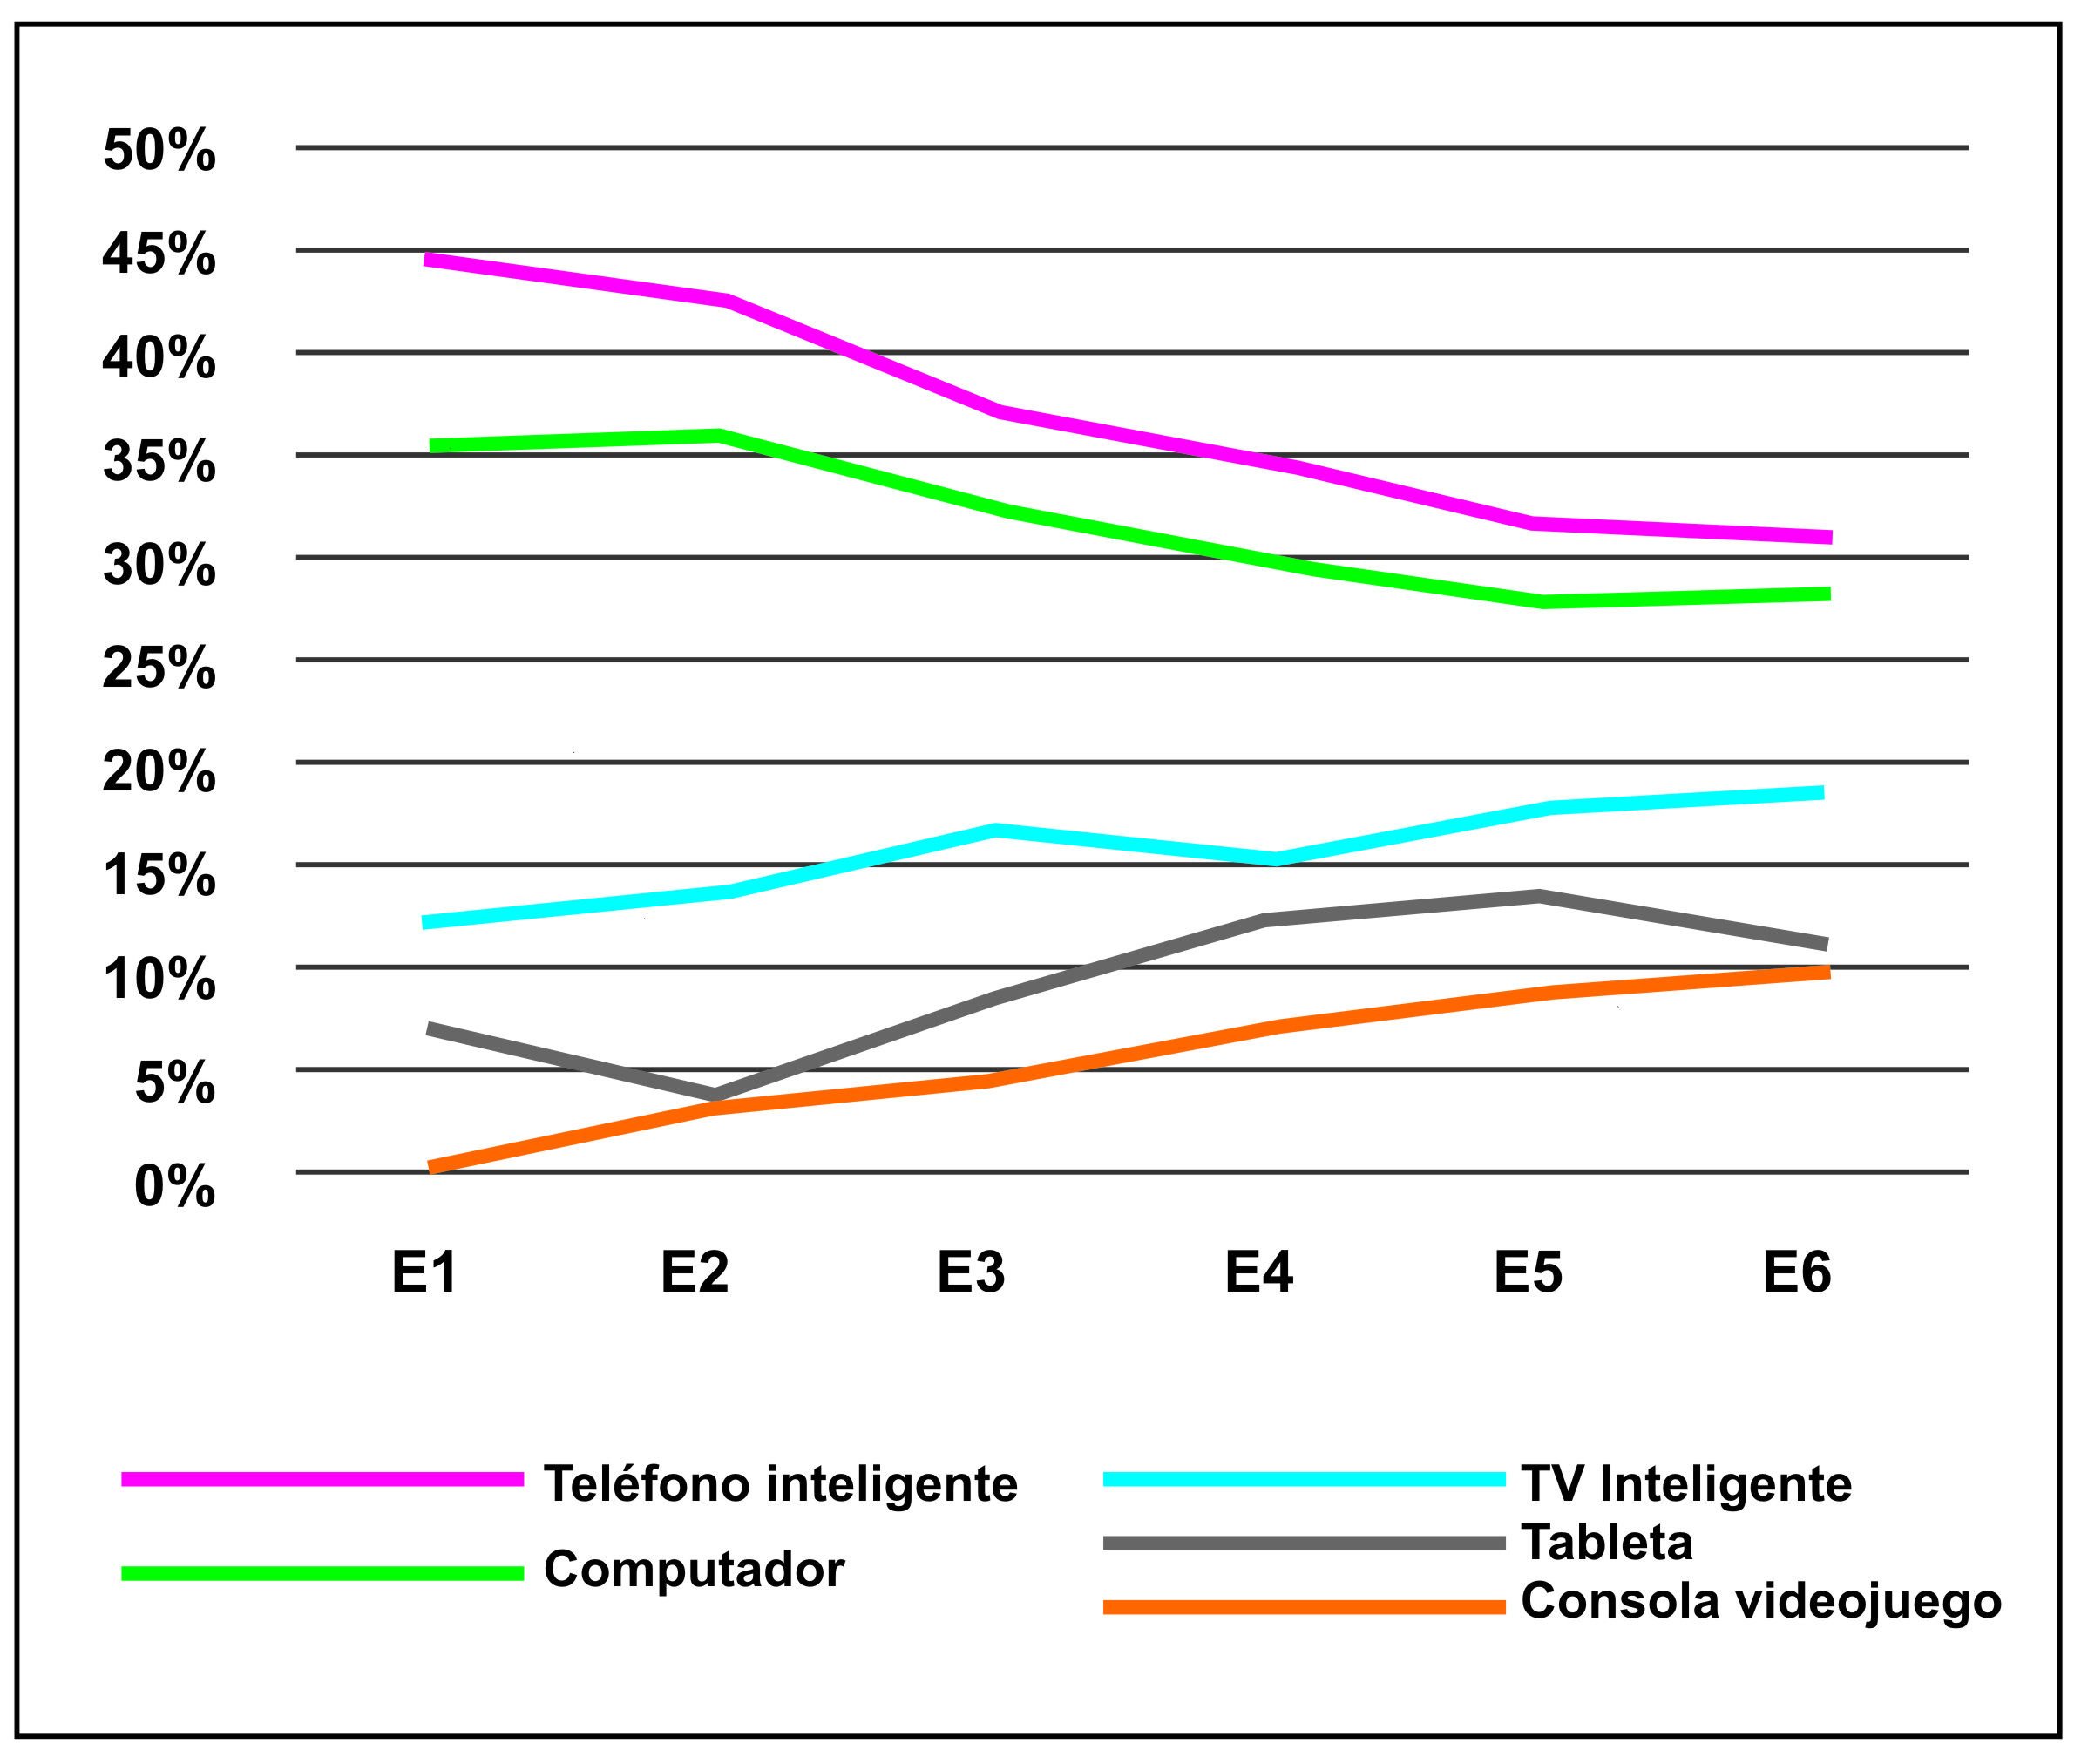
\includegraphics[width=0.6\textwidth]{fig1.jpg}
 \caption{Comparativo del uso de dispositivos para acceder a internet por cada estrato social.}
 \label{fig1}
 \source{Elaboración propia.}
\end{figure}

En lo que atañe al factor relacionado con el uso de internet para hacer reuniones virtuales, se encontró que las frecuencias dominantes de uso de internet para este propósito están en los rangos de 1 a 3 horas diarias y de menos de 1 hora por día. Para el caso del rango de uso diario de entre 1 y 3 horas, se tiene que en los estratos 1, 2 y 3 el porcentaje de hogares que manifiestan estar en reuniones virtuales es 30\%, 31.42\% y 31.14\%, respectivamente; en lo concerniente a los estratos 4, 5 y 6, los valores respectivos son de 28.54\%, 28.15\% y 39.29\% (ver \Cref{tab2}). Se destaca, de conformidad con estos resultados, que donde se encuentra un mayor número de respuestas dadas en relación al uso de internet para hacer reuniones virtuales entre 1 y 3 horas diarias, es en el estrato socio-económico más alto (el 6); el segundo valor que le sigue se aprecia en el estrato 2 (ver \Cref{fig2}).

\begin{table}[htpb]
\caption{Distribución de la utilización de internet para hacer reuniones virtuales.}
\label{tab2}
\centering
\begin{tabular}{lllllll}
\toprule 
Frecuencia / Estrato & 1 & 2 & 3 & 4 & 5 & 6
\\ 
\midrule
De 1 a 3 horas & 30,00\% & 31,42\% & 31,14\% & 28,54\% & 28,15\% & 39,29\%
\\
De 3 a 5 horas & 6,67\% & 10,18\% & 17,26\% & 18,54\% & 23,70\% & 10,71\%
\\
De 5 a 7 horas & 10,00\% & 9,29\% & 9,61\% & 15,12\% & 14,07\% & 14,29\%
\\
Más de 7 horas & 3,33\% & 11,06\% & 8,36\% & 13,41\% & 6,67\% & 7,14\%
\\
Menos de 1 hora & 36,67\% & 20,35\% & 19,93\% & 18,05\% & 21,48\% & 17,86\%
\\
Nada & 13,33\% & 17,70\% & 13,70\% & 6,34\% & 5,93\% & 10,71\%
\\ 
\bottomrule
\end{tabular}
\source{Elaboración propia.}
%\notes{Esta é uma nota exemplo que poderá, opcionalmente, ser adicionada a uma tabela ou figura.}
\end{table}

\begin{figure}[htbp]
 \centering
 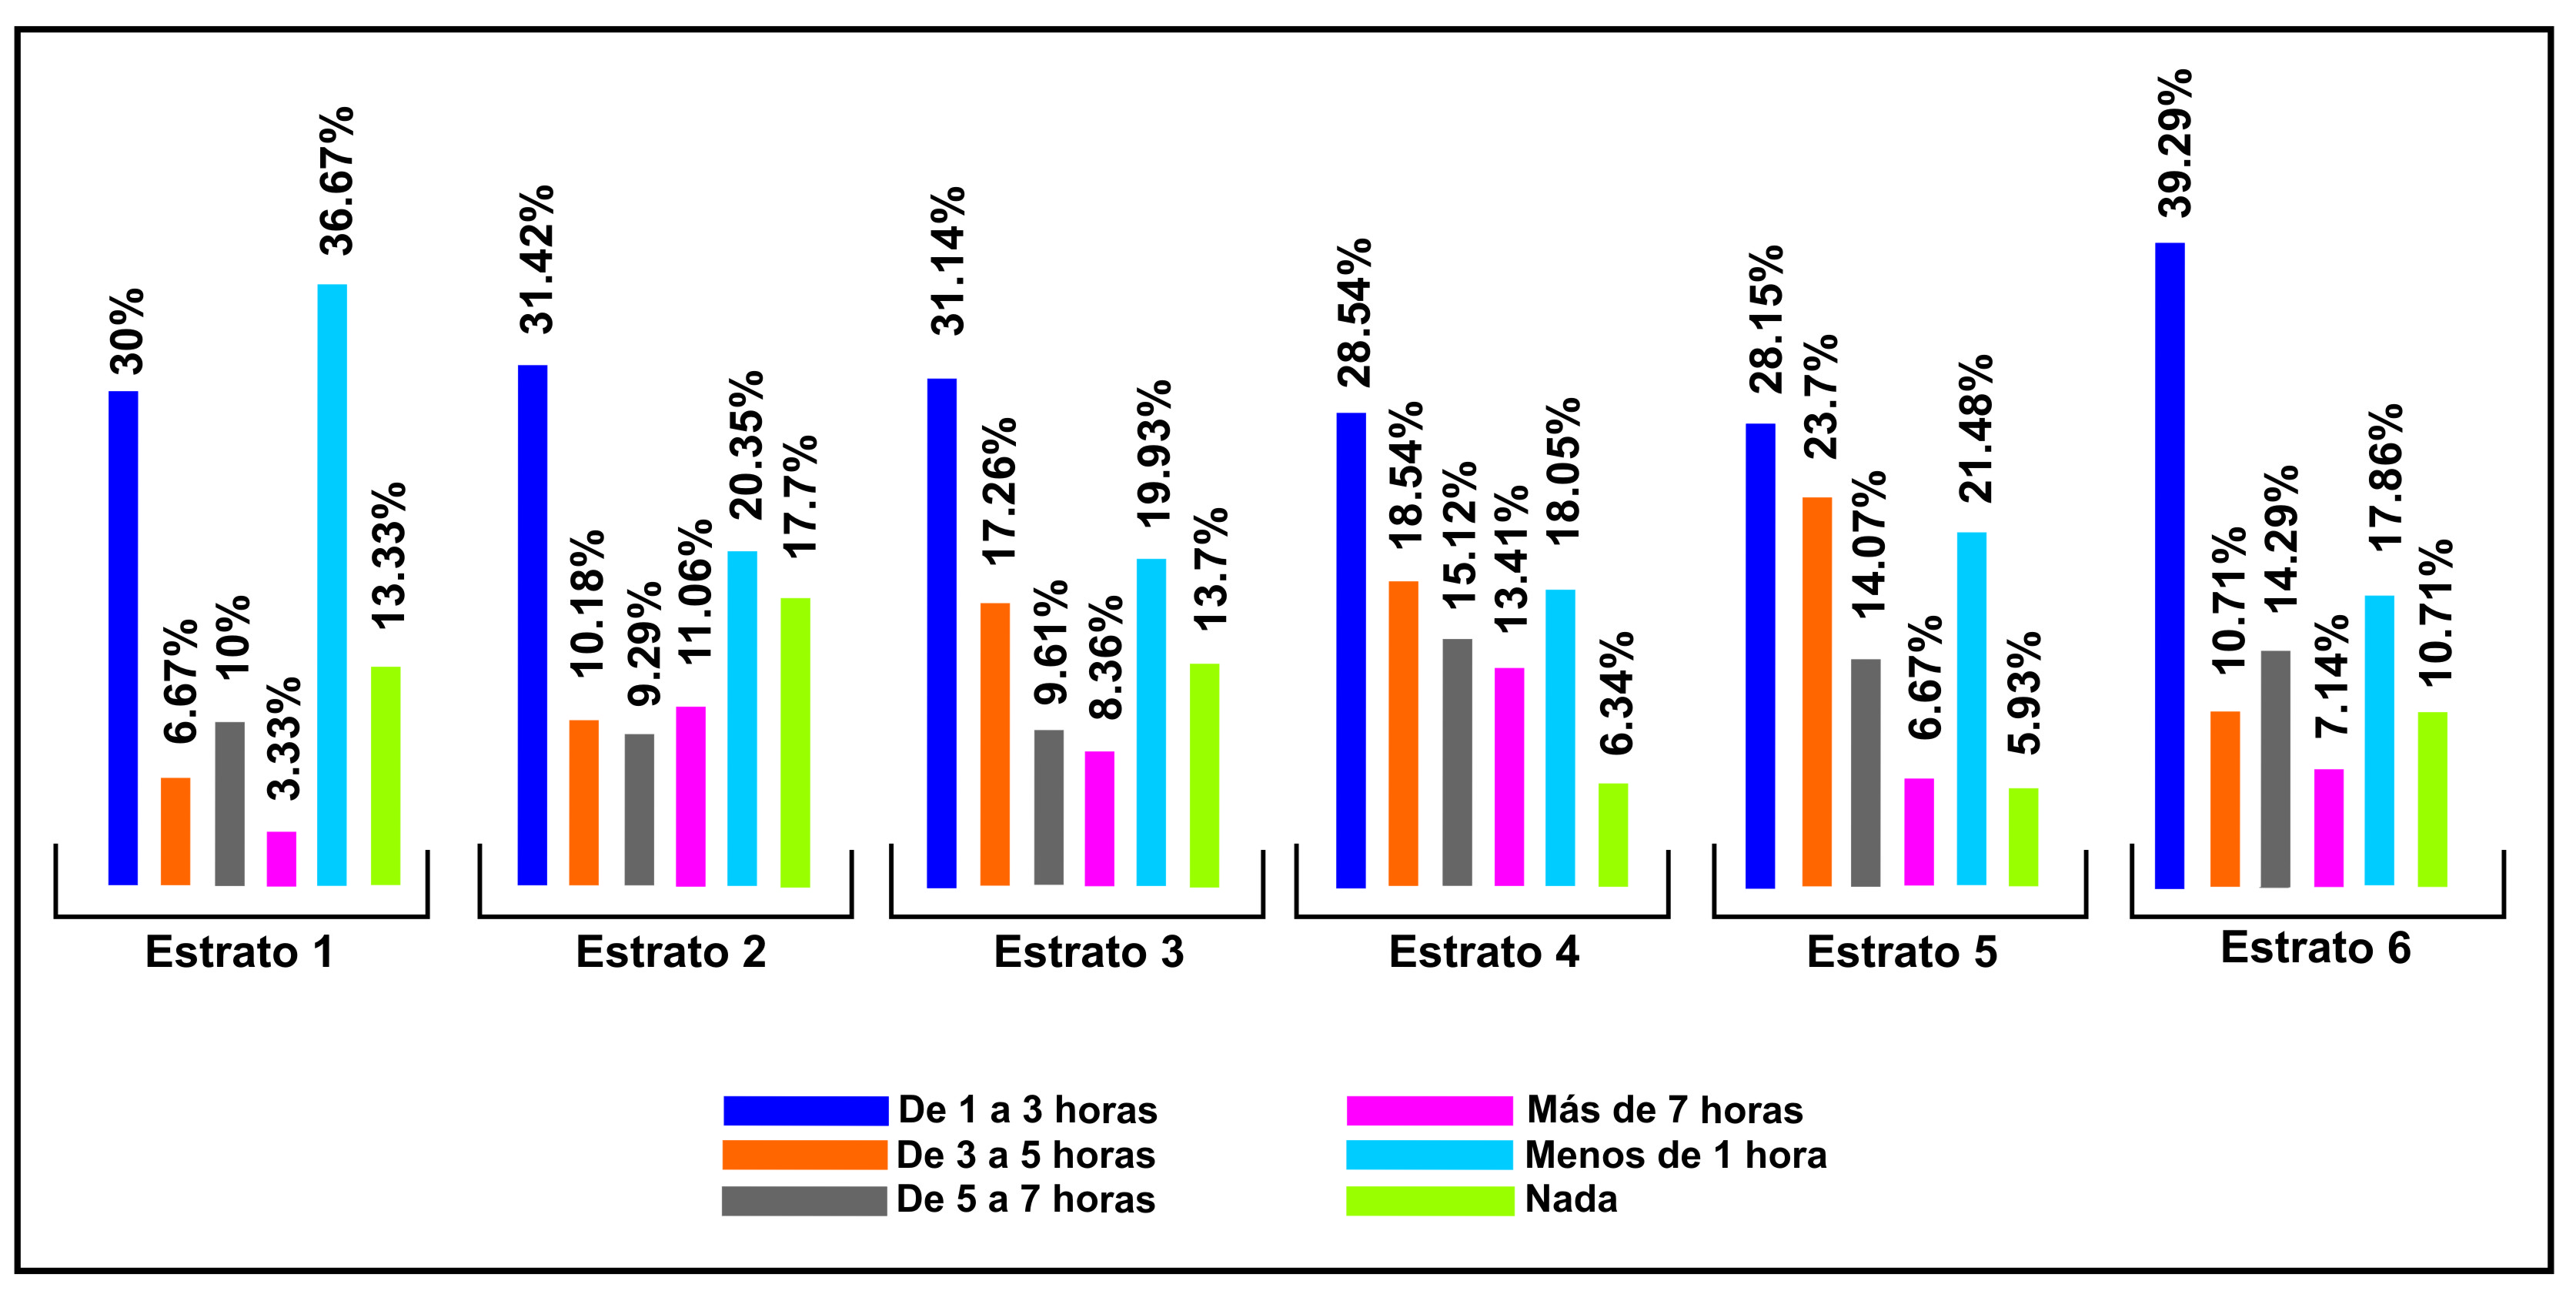
\includegraphics[width=0.9\textwidth]{fig2.jpg}
 \caption{Uso dado a la internet para reuniones virtuales (por día).}
 \label{fig2}
 \source{Elaboración propia.}
\end{figure}

\subsection{Consumo de redes sociales, radio y televisión}
Para efectos de contrastar la hipótesis que se planteó en el sentido de que existen diferencias significativas en el tiempo dedicado a usar las redes sociales Facebook, Twitter, Instagram, YouTube y Tik-Tok, considerando el estrato socio-económico de la población, se procedió a hacer un análisis de varianza (ANOVA) con dos o más factores, esto porque el tamaño de muestra de las combinaciones de tratamiento fue uniforme (segunda fase de aplicación de encuestas). Así, los análisis implicaron una idéntica descomposición de la suma de cuadrados dentro del modelo \cite{vallejo2010}. En la \Cref{tab3} se aprecia el resultado detallado por cada red social analizada, donde la muestra poblacional estuvo homogenizada en función de un valor n idéntico ($n = 135$) por cada estrato social observado.

\begin{table}[htpb]
\caption{Uso diario de las redes sociales en horas considerando la estratificación social.}
\label{tab3}
\centering
\begin{tabular}{llllllll}
\toprule 
& EST 1 & EST 2 & EST 3 & EST 4 & EST 5 & EST 6 & Total
\\ 
\midrule
FACEBOOK & & & & & &
\\
\arrayrulecolor[gray]{.7}
\midrule
Suma & 223 & 275,5 & 255,5 & 256 & 75,5 & 213,5 & 1399
\\
Promedio & 1,65185 & 2,04074 & 1,89259 & 1,896 & 1,3 & 1,58148 & 1,7271
\\
Varianza & 3,71744 & 4,72780 & 4,0835 & 4,4443 & 2,50447 & 5,52316 & 4,2017
\\
\arrayrulecolor{black}
\midrule
TWITTER & & & & & &
\\
\arrayrulecolor[gray]{.7}
\midrule
Suma & 53,5 & 103,5 & 115,5 & 126 & 96,5 & 85 & 580
\\
Promedio & 0,39629 & 0,76666 & 0,85555 & 0,9333 & 0,71481 & 0,6296 & 0,7160
\\
Varianza & 1,94438 & 2,43582 & 2,24577 & 2,9507 & 2,15873 & 2,27598 & 2,3506
\\
\arrayrulecolor{black}
\midrule
INSTAGRAM & & & & & &
\\
\arrayrulecolor[gray]{.7}
\midrule
Suma & 117,5 & 245,5 & 309 & 385,5 & 381 & 360 & 1798,5
\\
Promedio & 0,8703 & 1,81851 & 2,28888 & 2,8555 & 2,82222 & 2,66666 & 2,2203
\\
Varianza & 1,69762 & 3,83808 & 4,51666 & 6,4024 & 5,15845 & 6,9776 & 5,2285
\\
\arrayrulecolor{black}
\midrule
YOUTUBE & & & & & &
\\
\arrayrulecolor[gray]{.7}
\midrule
Suma & 242,5 & 298 & 286,5 & 295,5 & 350,5 & 297,5 & 1770,5
\\
Promedio & 1,79629 & 2,20740 & 2,12222 & 2,1888 & 2,59629 & 2,20370 & 2,1858
\\
Varianza & 2,26603 & 4,96412 & 4,00174 & 3,9398 &
4,12871 & 4,62050 & 4,0164
\\
\arrayrulecolor{black}
\midrule
TIK-TOK & & & & & &
\\
\arrayrulecolor[gray]{.7}
\midrule
Suma & 102,5 & 123,5 & 109,5 & 144,5 & 156 & 196 & 832
\\
Promedio & 0,75925 & 0,91481 & 0,81111 & 1,0703 & 1,15555 & 1,45185 & 1,0271
\\
Varianza & 1,47332 & 3,67739 & 2,2980 & 3,2729 & 4,58756 & 6,81669 & 3,7199
\\
\arrayrulecolor{black}
\bottomrule
\end{tabular}
\source{Elaboración propia.}
%\notes{Esta é uma nota exemplo que poderá, opcionalmente, ser adicionada a uma tabela ou figura.}
\end{table}

El análisis de varianza (ANOVA) indicó que las diferencias entre los promedios del tiempo diario dedicado al uso de las redes sociales (ver en \Cref{tab4}), fue significativo, y que, en efecto, la variable estrato social está relacionada con ese tiempo de consumo ($F(4, N = 135) = 98.924$; $f = 2.374$; $p < .001$). Al cotejar los resultados relacionados con el análisis de varianza de los tiempos de uso dado a las redes en función de los seis estratos sociales observados, se encontró una variación significativa ($F(5, N = 135) = 11.227$; $f = 2.216$; $p < .001$). Así mismo, se aprecia una significancia ($p < .001$) al analizar la interacción entre las variables tiempo de uso de las redes sociales y estrato social.

\begin{table}[htpb]
\caption{Análisis de varianza (ANOVA).}
\label{tab4}
\centering
\begin{tabular}{p{0.1\textwidth}p{0.1\textwidth}p{0.12\textwidth}p{0.12\textwidth}p{0.1\textwidth}p{0.12\textwidth}p{0.12\textwidth}}
\toprule 
& Suma de cuadrados & Grados libertad & Cuadrados   (promedio) & F & Probabilidad & Valor crítico para F
\\ 
\midrule
Muestra & 1499,03 & 4 & 374,75 & 98,924 & 0,000 & 2,374142409
\\
Columnas & 212,66 & 5 & 42,53 & 11,227 & 0,000 & 2,216323178
\\
Interacción & 347,72 & 20 & 17,38 & 4,589 & 0,000 & 1,573141491
\\
Grupo & 15229,11 & 4020 & 3,78 & & &
\\
Total & 17288,53 & 4049 & & & &
\\ 
\bottomrule
\end{tabular}
\source{Elaboración propia.}
%\notes{Esta é uma nota exemplo que poderá, opcionalmente, ser adicionada a uma tabela ou figura.}
\end{table}

De otra parte, en el momento de cotejar las hipótesis planteadas en el sentido de asumir el consumo de ciertas redes sociales como mayor en relación a otras, lo mismo que el consumo de televisión on-line (en línea) con respecto a la escucha de radio vía internet, se procedió a hacer un análisis del tipo \emph{prueba pareada}, dado que se deseaba revisar que las diferencias observadas fueran el resultado de las características de las redes sociales cotejadas. Esto supuso hacer la comparación entendiendo que podrían hacer presencia varias fuentes de variabilidad explícitas \cite{gutierrez_pulido2012, montilla2010}. En ese orden de ideas, se tomaron los valores dados por los 1419 sujetos encuestados, y se procedió a hacer las correspondientes comparaciones estadísticas en relación al tiempo diario de uso de las redes sociales.

Los siguientes son los resultados, tal y como se puede apreciar en la \Cref{fig3}: con respecto a la comparación entre Facebook e Instagram, se encuentra que hay mayor tiempo de consumo en horas diarias en favor de la red Instagram ($M = 2.293$; $DE = 5.51$; valores de la red Facebook: $M = 1.786$; $DE = 4.2$; $t(1418) =  7.61$; $p = .000$). También se encuentra un mayor tiempo de uso de la red Instagram en comparación con el uso de YouTube ($M = 2.127$; $DE = 4.32$; $t(1418) = 2.847$; $p = .002$). Por su parte, cuando se compara el tiempo de uso de YouTube con respecto a la red Tik-Tok ($M = 0.939$; $DE = 3.54$; $t(1418) = 19.681$; $p = .000$), se encuentra una diferencia significativa en favor del canal de contenidos audiovisuales. Por último, al cotejar el tiempo de uso de Tik-Tok contra el tiempo destinado a la red Twitter ($M = 0.879$; $DE = 2.88$; $t(1418) = 1.097$; $p = .136$), se encuentra una diferencia en favor de la red Tik-Tok, pero que no es estadísticamente significativa.

\begin{figure}[htbp]
 \centering
 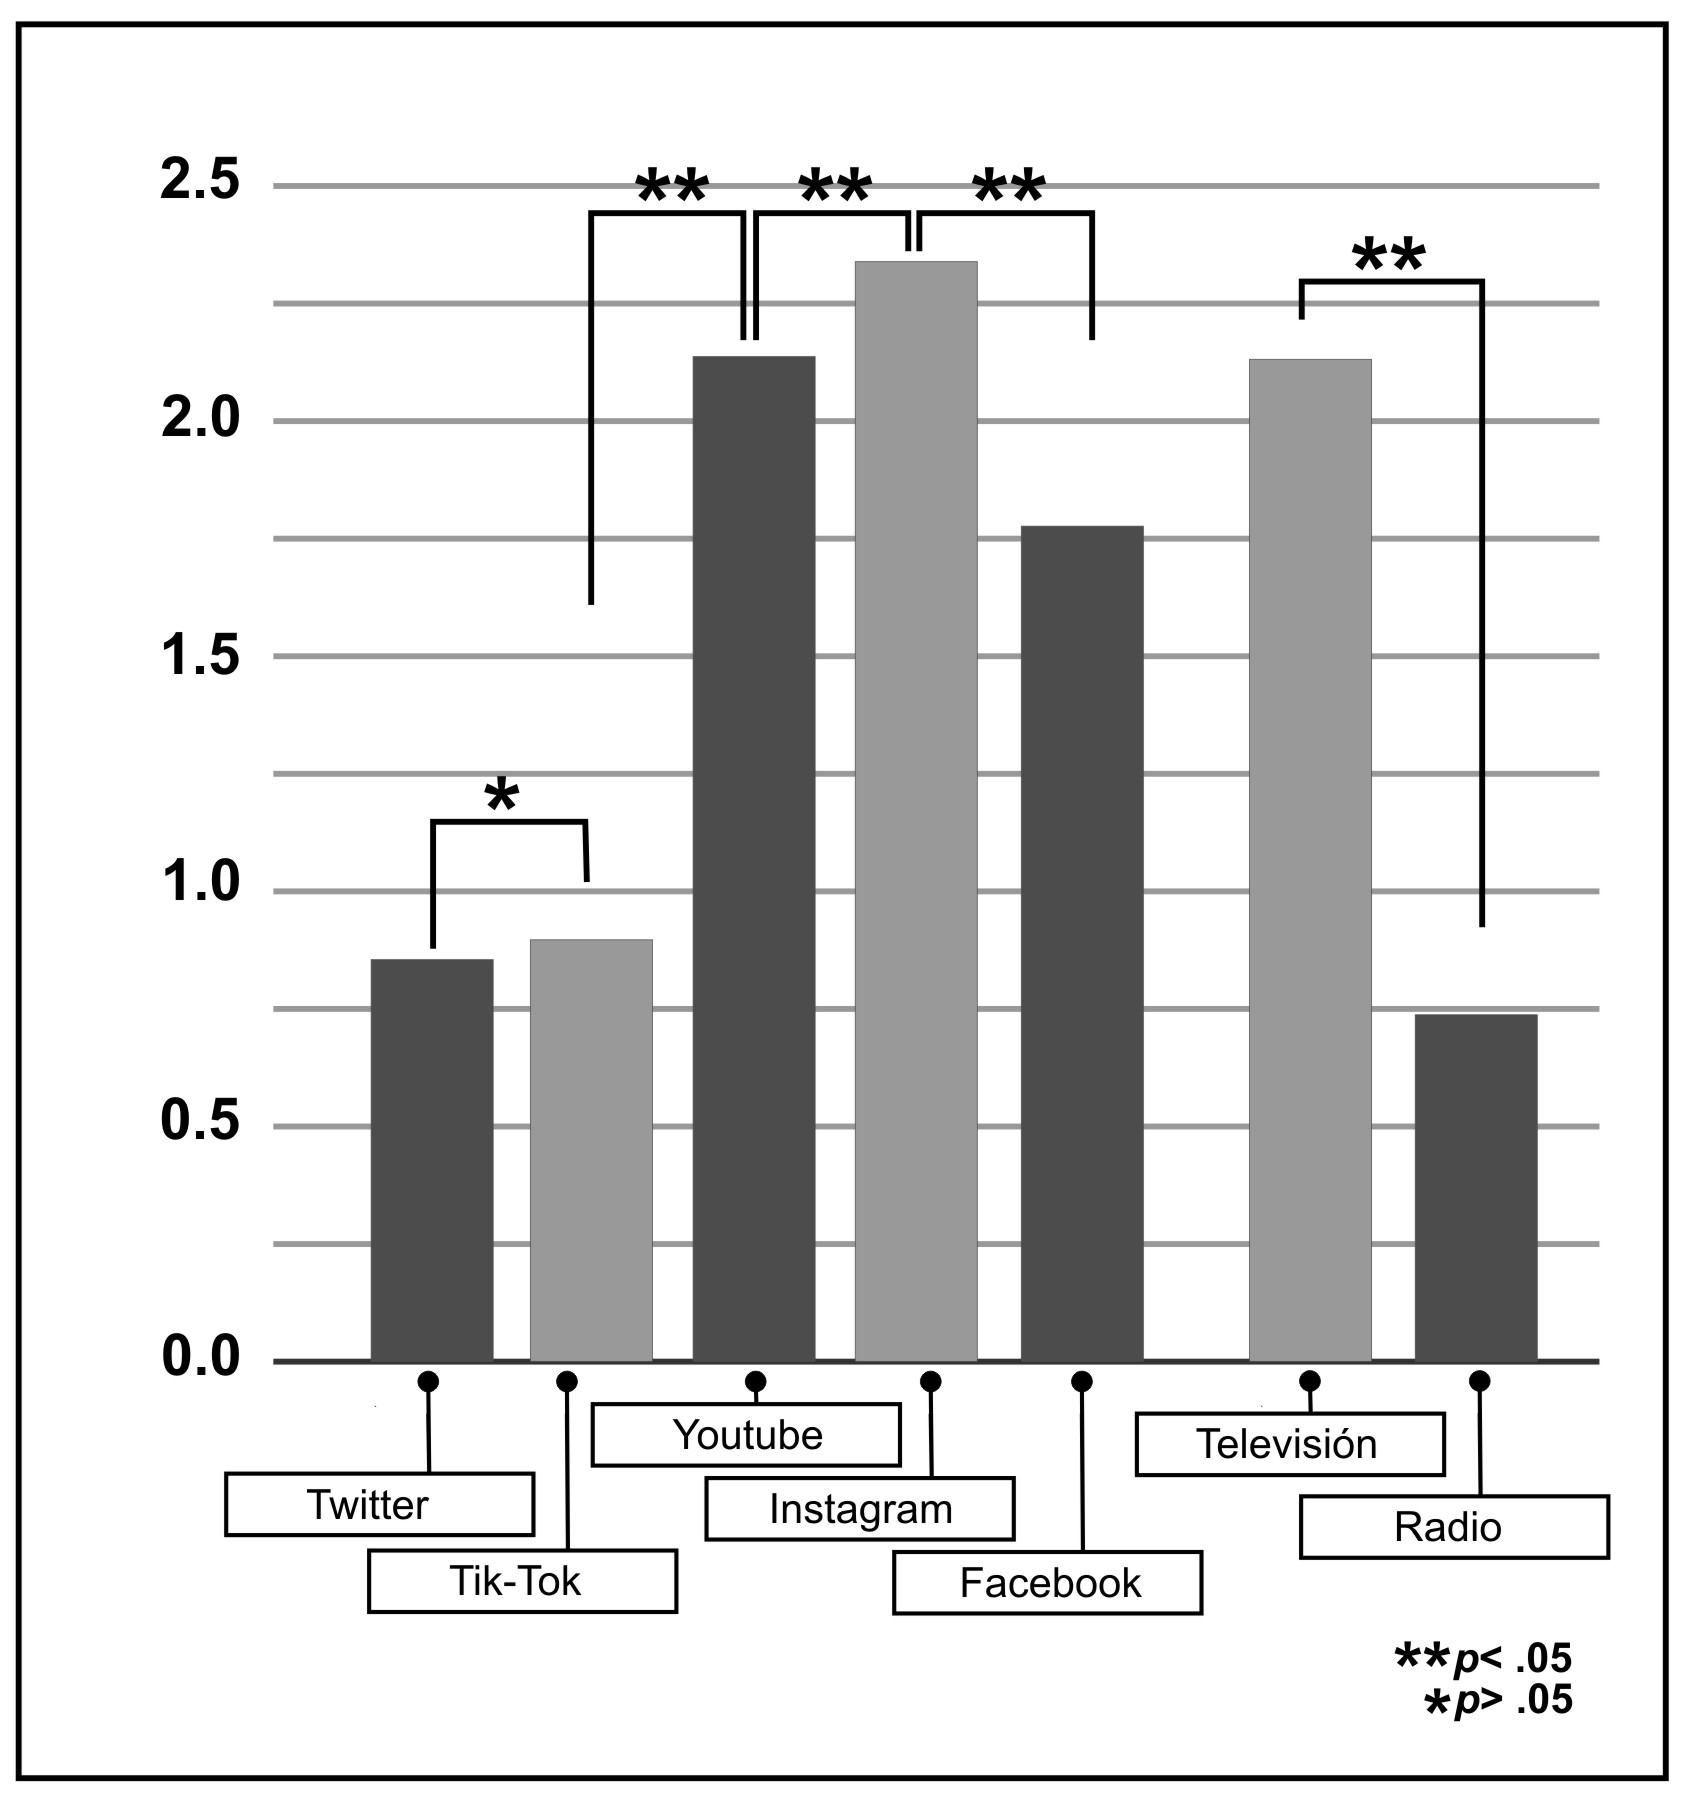
\includegraphics[width=0.7\textwidth]{fig3.jpg}
 \caption{Comparativo del tiempo en horas utilizado para estar en redes sociales y para acceder a contenidos televisivos y radiales.}
 \label{fig3}
 \source{Elaboración propia.}
\end{figure}

Tal y como se aprecia en la \Cref{fig3}, el consumo de contenidos televisivos a través de internet ($M = 2.06$; $DE = 3.65$) es mayor que el consumo de la radio vía web ($M = 0.74$; $DE = 1.81$). Esta diferencia en favor de la televisión es significativa ($t(1418) = 24.02$; $p = .000$).

\section{Discusión y conclusiones}
Este estudio muestra que el uso de los teléfonos inteligentes para acceder a la internet prevalece sobre otro tipo de dispositivos. El nivel de penetración de los teléfonos celulares ha logrado abarcar diversos segmentos poblacionales, esto porque existe una amplia oferta, diversidad de marcas y opciones de precio \cite{mongardini2020}, hecho que hace de estos dispositivos una herramienta útil para los trabajadores de diferentes segmentos poblacionales \cite{agger2011}. Según los resultados obtenidos en este estudio, se encuentra que quienes más emplean el celular para acceder a la web (internet) son los jóvenes pertenecientes al estrato más bajo, esto es, al estrato 1 (44.6\%), seguidos por el estrato 2 (42.9\%).

De acuerdo con \textcite{anaya_figueroa2021}, una manera de acortar la brecha tecnológica entre segmentos poblacionales económicos es mediante la generación de oportunidades para acceder a los dispositivos y tecnologías por los cuales navegar en la internet. Es así como el uso de los teléfonos inteligentes se ha convertido en una alternativa plausible para los segmentos socio-económicos bajos, pero sin que esto suponga una solución definitiva, porque la versatilidad que tiene un teléfono para sacar el máximo provecho de los contenidos que se encuentran disponibles en internet no necesariamente es igual a la de un computador, llámese portátil o del tipo desktop (escritorio), pues existen diferencias de usabilidad y de desempeño del usuario dependiendo del dispositivo usado \cite{ha2020}. Acótese, sin embargo, que ciertos contenidos están diseñados más para un acceso desde móviles inteligentes que desde ordenadores \cite{kelton2020}, como es el caso de algunas redes sociales \cite{arkansyah2021}, más otros medios alternativos de interacción, como es el caso de la realidad aumentada \cite{li2020}, que resulta muy útil para que jóvenes y niños puedan interactuar en contextos digitales \cite{yadav2020}.

Los resultados muestran que desde los estratos 3 hasta el 6, el uso del móvil inteligente para acceder a internet oscila entre valores que van del 37.4\% (estrato 3) al 31.3\% (estrato 6), mientras que para los estratos 4 y 6 los porcentajes se corresponden a 34.7\% y a 31.5\%, respectivamente. Al cotejarse esta información con el acceso a internet mediante el uso de computadores, se observa que para los sujetos que pertenecen al estrato 1, este fue el segundo dispositivo más usado, luego del teléfono inteligente. Al comparar todos los estratos, se encuentra que el estrato más alto, el 6, es el que menos uso hace de ordenadores para acceder a internet.

Empero, sobresale que el porcentaje referido al uso del computador va decreciendo conforme aumenta la estratificación social (ver \Cref{fig1}). Lo opuesto sucede con los SmartTV (televisores inteligentes), pues se aprecia un mayor uso de este tipo de dispositivos en los estratos más altos que en el segmento más bajo (18.8\% contra 12.5\%). Como se puede apreciar en la \Cref{fig1}, y también en consonancia a los valores porcentuales expresados en la \Cref{tab1}, la curva de crecimiento porcentual en relación al uso de televisores, en concordancia con el aumento en la estratificación social, sólo presenta una baja entre los estratos 3 y 4, pero para los estratos 5 y 6 la curva vuelve a ser creciente, al punto de que, como se acotó previamente, el estrato más alto presenta la mayor tasa de consumo de internet por la vía del uso de televisores inteligentes.

En consonancia con lo que plantean \textcite{nunez2018}, la televisión ha sido uno de los medios masivos por excelencia, por su cobertura y penetración doméstica. Ese hecho no se ha modificado por la migración que han tenido los contenidos audiovisuales a las plataformas digitales; por el contrario, ha implicado una nueva posibilidad para hacer que todos los públicos accedan paulatinamente a una diversidad de información, donde los contenidos on-line (en línea) se integran a la televisión, configurando una experiencia particular en los usuarios \cite{harwig2000}.

Parecido a los televisores inteligentes pasa con las tabletas, en el sentido de que su uso es más dado en estratos altos que en los bajos. Según los resultados, las tabletas están en la cuarta posición en cuanto a la preferencia en uso de dispositivos para acceder a la internet. Como se ilustra en la \Cref{fig1}, se evidencia un incremento en el uso de este tipo de dispositivos conforme aumenta la estratificación social de los usuarios. Hecho similar se da con ocasión del uso de consolas de video juego, pues su uso se va incrementando progresivamente desde los estratos bajos hacia los altos (se pasa de un valor nulo en el estrato 1 hasta un valor porcentual máximo encontrado en el estrato 5, de 13.7\%). En efecto, existen estudios donde se analiza el uso de celulares, video juegos y tabletas como dispositivos que operan como medio de navegación en internet, donde se encuentra que se da un consumo marcado de estos dispositivos desde segmentos socio-económicos medios en ciudades principales de Colombia \cite{aristizabal2020}.

La adquisición de este tipo de dispositivos supone un esfuerzo económico para hogares del segmento medio, pero no para quienes están por encima de ese segmento, como también sucede en otros países \cite{lareau2003, vincent2007}. Al cotejar esta información con los resultados, se encuentra una coherencia, pues el uso de tabletas para navegar en internet se incrementa en los estratos 4 y 5 con respecto a los segmentos 1, 2 y 3, aunque se evidencia que el estrato 6 no supera el consumo de este dispositivo en relación al 5.

Los hallazgos también están en línea con la tendencia a encontrar un mayor acceso a las consolas de video juego para interactuar y navegar en internet por parte de segmentos poblacionales de mejores ingresos: en el estrato 1 no se reporta uso alguno de este tipo de dispositivos, mientras que en el estrato 6 prácticamente se duplica con relación al uso dado por el estrato medio de nivel 3 (ver \Cref{fig1}). La brecha tecnológica referida a dispositivos para acceder a la internet se hace manifiesta, donde los segmentos medios deben hacer esfuerzos por acceder a los dispositivos con respecto a quienes gozan de mejores niveles de poder adquisitivo \cite{aristizabal2020, lareau2003, vincent2007}. A nivel del uso de video-consolas, es posible evidenciar también una brecha que, inclusive, puede estar marcada por las diferencias socio-culturales que se dan entre las estratificaciones sociales, donde aspectos asociados al desarrollo cognoscitivo, cultural y perceptual de los individuos inciden en la manera de apropiarse e interactuar con estos dispositivos, configurando así otro tipo de brecha, esta vez en función del desarrollo cognitivo diferencial que se da entre segmentos socio-económicos dispares \cite{del_villar_munoz2006}.

Estos resultados suponen implicaciones en relación a los modos en que se pueden cerrar (o al menos acortar) las brechas tecnológicas entre estratos sociales, dado que la penetración que han logrado tener los teléfonos inteligentes y otros dispositivos en los diversos segmentos poblacionales ha permitido que se expanda el acceso a internet. Sin embargo, debe considerarse que, dependiendo del tipo de tarea o actividad que se quiere llevar a cabo mediante la navegación en internet, la funcionalidad del aparato utilizado podrá ser óptima o no, esto porque cada dispositivo tiene sus ventajas y desventajas, según el propósito por el que se accede a la red digital. En ese orden de ideas, emergen imperativos para atender la problemática, donde no se trata únicamente de brindar posibilidades a nivel del acceso a dispositivos tecnológicos, sino también de generar una coherencia entre el dispositivo y el propósito de su uso, todo ello ligado a una conectividad de calidad. La disparidad en el acceso a los dispositivos que se requieren para atender cada necesidad específica hace que se presente una brecha, lo que, a su vez, conlleva a diferencias tanto en el desarrollo cognoscitivo de los diferentes segmentos poblacionales \cite{del_villar_munoz2006}, como en la calidad de la educación, dependiendo también de si se tienen o no los recursos necesarios para una apropiada conectividad \cite{lopez2020}.

Con respecto al uso de internet para hacer reuniones virtuales, se aprecia que las frecuencias que prevalecen están en los rangos de 1 a 3 horas diarias y de menos de 1 hora por día. Para el caso del rango de uso diario de entre 1 y 3 horas, se tiene que en los estratos 1, 2 y 3 el porcentaje de encuestados que hacen reuniones virtuales oscila entre el 30\% y el 31.14\%. En estratos 4, 5 y 6, los valores respectivos son de 28.54\%, 28.15\% y 39.29\%. Casi 10 puntos porcentuales separan al estrato 6 del 1, pero se encuentra mucha similitud entre los valores del estrato 1 con los de los estratos 4 y 5. Según estos datos, no es posible evidenciar un efecto claro (de tipo descriptivo) del nivel socio-económico sobre el tiempo dado a las reuniones virtuales. Sin embargo, el rango dado entre 1 y 3 horas es diario, y si se multiplica por 5 días laborales, o por la totalidad de los días de la semana, se puede pensar en duraciones que pueden llegar a las 15 o 21 horas semanales. Este hecho puede estar relacionado con el incremento que han venido experimentando las reuniones virtuales, en razón a los confinamientos derivados de la contingencia sanitaria de la Covid-19 \cite{antonello2020, karl2021}.

Debe ser subrayado que se está aludiendo a una población que está entre los 18 y los 24 años de edad. En ese sentido, puede existir un potencial uso de la red relacionado con aspectos académicos, laborales, o de mera interacción por razones de tipo personal \cite{danna2020}, que pueden también estar asociados con las necesidades psico-sociales de los jóvenes \cite{tomek1999, notley2009}.

De otra parte, en lo relativo al uso de las redes sociales, se encontró que existe un efecto significativo de la variable socio-económica (estrato social) sobre el tiempo dedicado a ellas por parte de los encuestados. Los resultados indicaron que las diferencias entre los promedios del tiempo diario dedicado al uso de redes sociales son significativas. Se concluye que el factor estrato social está relacionado con la duración en tiempo dada al uso de redes sociales. También se encontró significancia estadística al analizar la interacción entre las variables \emph{tiempo de uso de las redes sociales} y \emph{estrato social}.

Al tomar muestras idénticas por cada uno de los seis segmentos poblacionales, se encuentra que los promedios de uso dependen de cada red social. Sobresale cómo para las redes sociales analizadas, el tiempo de uso diario en el estrato 1 en todos los casos es menor que en los demás (ver en \Cref{tab3}). En el caso de YouTube, sucede que el promedio del estrato 2 (2.207 horas diarias) está equiparado al tiempo dado por los estratos 5 y 6 (2.203 y 2.185 horas diarias respectivamente), y que para las redes Twitter y Facebook, los tiempos son superiores en los estratos 2, 3 y 4, frente a los usuarios de los estratos 5 y 6 (ver \Cref{tab3}). Para la red Instagram, los mayores promedios de consumo diario en horas está en los estratos 3 y 4 (2.855 y 2.822, respectivamente). Este hecho marca una diferencia con lo que sucedía hacia el año 2013, donde la diferencia entre el estrato 1 y el 6 era casi seis veces mayor en favor de los más pudientes, o donde estratos 1 y 2 tomados en conjunto eran superados cuatro veces por los estratos 5 y 6 agregados \cite{narvaez_montoya2013}. Desde los resultados presentados, puede verse una diferencia dependiendo del tipo de contenido o red que se analice, pero se remarca en todo caso que el factor socio-económico sí entra en juego, en términos generales, como un factor que incide en el acceso a internet para usar redes sociales (ver \Cref{tab4}).

En relación a los análisis de la diferencia entre el uso de cada red (considerando la muestra total de 1419 participantes), en efecto se encontraron diferencias significativas entre el uso en horas dado a redes sociales, por una parte, y al consumo entre contenidos radiales y televisivos, por otra. Sea estimado que acá no se considera el factor socio-económico, sino que se revisa en general la preferencia dada a cada red social y a los contenidos televisivos y radiales, indagando sobre las diferencias significativas encontradas (ver en \Cref{tab3}).

Considérense las diferencias significativas: mayor consumo de Instagram sobre Facebook ($t(1418) =  7.61$; $p = .000$). Puede atribuirse a que en situación de pandemia los jóvenes están en sus hogares con su familia, hecho que no implicaría uno de los usos esenciales de la red Facebook, que es mantenerse conectado con la familia \cite{arcilacalderon2017}. En cambio, Instagram suele implicar la necesidad de conexión con amigos, enterarse de noticias y buscar material para entretenerse, como videos y música \cite{ting2015}. Segunda diferencia significativa: mayor consumo de Instagram sobre YouTube ($t(1418) = 2.847$; $p = .002$). La razón puede centrarse en que Instagram tiene una posibilidad de cargar y compartir información con inmediatez y posibilidad de transmisión práctica, dirigida a una red de amigos en particular \cite{ting2015}.

Otra diferencia significativa fue el mayor consumo de YouTube sobre Tik-Tok ($t(1418) = 19.681$; $p = .000$). Se pudo haber esperado un resultado contrario. La red Tik-Tok es muy usada por los jóvenes por su talante lúdico, expresivo y creativo \cite{shutsko2020}). Sin embargo, puede presumirse que, dado que YouTube implica la observación de videos de media o larga duración, los tiempos de visita a ese canal podrán ser, en promedio, mucho más extensos que los contenidos generados en la red Tik-Tok. Esto puede explicarse también por el carácter tutorial que se le imputa al canal YouTube, y por los extensos videos que allí se pueden observar con fines de entretención \cite{asselin2011}. Por último, mencionar que el consumo de contenidos televisivos vía internet ($M = 2.06$; $DE = 3.65$) fue mayor que el consumo de la radio por esa misma vía ($M = 0.74$; $DE = 1.81$). Esta diferencia en favor de la televisión resultó ser significativa ($t(1418) = 24.02$; $p = .000$). El lenguaje video-gráfico prima, hecho que no sorprende si se consideran las ventajas que el formato audiovisual tiene por sus posibilidades en términos de transmisión de información y de generación de emociones y experiencias significativas \cite{kalliris2014}.

En línea con lo anterior, deben señalarse diversas implicaciones. En primera instancia, el reconocimiento de la incidencia que tiene el nivel socio-económico del usuario sobre el uso de redes sociales. A su vez, contemplar que ciertas plataformas pueden tener un consumo similar, en estratos dispares, como es el caso del canal YouTube, en relación al comparativo entre su consumo en estrato 2 frente a los estratos 5 y 6. Dado que cada red social y cada plataforma provee contenidos y experiencias de usuario distintas, factores psicográficos entran a jugar un papel decisivo a la hora de preferir una plataforma en específico \cite{rodriguez2018}. Esto supondría que el uso de redes sociales no sólo se ve influenciado por la condición socio-económica, sino por la relación existente entre la experiencia del usuario y sus expectativas, según su estilo de vida. El modo en que se accede a Internet y el uso dado a la web en función del consumo de redes sociales son aspectos que se definen sobre la base de ciertas condiciones necesarias para el acceso más preferencias y expectativas personales frente al uso de los dispositivos, plataformas y redes sociales. También se puede entrever la variación en el consumo de redes como Instagram, cuando se coteja con estudios predecesores realizados en años anteriores a la pandemia. Esto puede tener también una implicación en cuanto a la forma en que ciertas tecnologías se van haciendo mas asequibles, lo que posibilita una mayor masificación de las mismas.

Lo anterior pone en evidencia diversas limitaciones del estudio acá reportado. Primero, no se hace un análisis multivariado para cotejar la potencial incidencia de diversos aspectos demográficos y psicográficos sobre el consumo de Internet. En ese orden de ideas, nuevas investigaciones podrían hacerse, cotejando otros factores para establecer diversas relaciones entre los diferentes factores intervinientes. En segundo término, hay una limitación en lo que refiere a la potencial representatividad de los datos, dado que el muestreo utilizado fue de tipo no probabilístico. Para seguir haciendo acopio de nueva información en relación al uso de internet y el consumo de medios y de redes sociales, otras investigaciones tendrán que llevarse a cabo, considerando otras posibilidades para la selección de la muestra, donde se apele a muestreos probabilísticos. Se podrá también implementar modelos como el muestreo estratificado, formando grupos homogéneos y heterogéneos, según las características por las cuáles se quieran tipificar los grupos objeto de estudio. Prospectivamente, también se podrá hacer investigación basada en un muestreo de conglomerados, involucrando así una selección de grupos, buscando con ello complejizar el abordaje del consumo de medios e internet en función de otras variables como las zonas geográficas, las creencias religiosas, más otros factores de tipo demográfico y psicográfico que aporten en la observación del fenómeno. De otra parte, este estudio, por ser transversal, debe asumirse como limitado, entendiendo que la contingencia sanitaria ocasionada por la Covid-19 se ha extendido por muchos meses, hecho que obliga a que a futuro se hagan nuevos estudios para revisar las diversas obervaciones hechas al fenómeno a nivel Colombia y a nivel región, más la posibilidad de proponer investigaciones longitudinales cuando emerjan nuevas circunstancias macro-ambientales que puedan impactar en conductas relacionadas con el consumo de información, medios e internet.

Para cerrar, por lo analizado en el presente estudio, se concluye que el factor socio-económico sí incide en el consumo de internet y de redes sociales en la población juvenil colombiana, y que existen variaciones significativas entre el consumo de varias de las redes sociales cotejadas. El contenido televisivo supera al contenido radial, cuando de acceder a estos contenidos por internet se trata. Existen preferencias hacia unas redes sociales por sobre otras, al punto de que es posible hablar de redes más usadas por cada uno de los diferentes estamentos socio-económicos analizados, no siempre siendo los estratos altos los que más uso hacen de cada red. Esto supone una relativización que necesariamente debe considerarse en el momento de hacer referencia a la llamada brecha tecnológica entre grupos poblacionales socio-económicos de la sociedad colombiana.

\printbibliography\label{sec-bib}
% if the text is not in Portuguese, it might be necessary to use the code below instead to print the correct ABNT abbreviations [s.n.], [s.l.]
%\begin{portuguese}
%\printbibliography[title={Bibliography}]
%\end{portuguese}


%full list: conceptualization,datacuration,formalanalysis,funding,investigation,methodology,projadm,resources,software,supervision,validation,visualization,writing,review
\begin{contributors}[sec-contributors]
\authorcontribution{Guillermo Rodríguez-Martínez}[formalanalysis,methodology,writing,review]
\authorcontribution{Carlos Andrés Arango Lozano}[datacuration,projadm,visualization]
\end{contributors}

\appendix 
\section*{Encuesta aplicada}\label{apen}
Introducción: Reciba un saludo. Agradecemos su participación voluntaria en el diligenciamiento de este formulario. La Universidad Jorge Tadeo Lozano agradece el tiempo que usted dispondrá para diligenciar las siguientes preguntas. Recuerde que todos los datos serán tratados de conformidad a las regulaciones dispuestas en nuestro país.

\begin{enumerate}
    \item Edad:
    \item Sexo:
    \begin{enumerate}
        \item Masculino
        \item Femenino
    \end{enumerate}
    \item Ciudad o población en donde reside:
    \item ¿Es usted residente colombiano?
    \begin{enumerate}
        \item Si
        \item No
    \end{enumerate}
    \item Nivel Socio-económico (indique su estrato social):
    \item Señale los dispositivos tecnológicos que tiene en casa en el momento actual (puede marcar más de una opción):
    \begin{enumerate}
        \item Computador de escritorio
        \item Computador portátil
        \item Tableta o iPad
        \item Teléfono móvil con conexión a Internet (Smartphone)
        \item Teléfono móvil sin conexión a Internet
        \item Televisión sin conexión a Internet
        \item Televisión con conexión a Internet (Smart-TV)
        \item Consolas de videojuegos
    \end{enumerate}
    \item Señale con qué dispositivo/s se conecta a Internet y a las redes sociales en la actual situación de confinamiento (puede señalar más de una opción).
    \begin{enumerate}
        \item Computador
        \item Teléfono con datos (Smartphone)
        \item Tableta o iPad
        \item Televisión con Internet (Smart-TV)
        \item Consola de videojuegos
    \end{enumerate}
    \item En la situación actual de confinamiento, señale la frecuencia diaria con la que utiliza los siguientes Medios de Comunicación e Información vía Internet (contestar todas las filas).
   
    Radio:
    \begin{enumerate}
        \item Nada
        \item Menos de 1 hora
        \item De 1 a 3 horas
        \item De 3 a 5 horas
        \item De 5 a 7 horas
        \item Más de 7 horas
    \end{enumerate}
    
    Televisión:
    \begin{enumerate}
        \item Nada
        \item Menos de 1 hora
        \item De 1 a 3 horas
        \item De 3 a 5 horas
        \item De 5 a 7 horas
        \item Más de 7 horas
    \end{enumerate}
    \item En la situación actual de confinamiento, señale la frecuencia diaria con la que utiliza las siguientes redes sociales (contestar todas las filas).
    
    Facebook:
    \begin{enumerate}
        \item Nada
        \item Menos de 1 hora
        \item De 1 a 3 horas
        \item De 3 a 5 horas
        \item De 5 a 7 horas
        \item Más de 7 horas
    \end{enumerate}
    
    Twitter:
    \begin{enumerate}
        \item Nada
        \item Menos de 1 hora
        \item De 1 a 3 horas
        \item De 3 a 5 horas
        \item De 5 a 7 horas
        \item Más de 7 horas
    \end{enumerate}
        
    Instagram:
    \begin{enumerate}
        \item Nada
        \item Menos de 1 hora
        \item De 1 a 3 horas
        \item De 3 a 5 horas
        \item De 5 a 7 horas
        \item Más de 7 horas
    \end{enumerate}
    
    YouTube:
    \begin{enumerate}
        \item Nada
        \item Menos de 1 hora
        \item De 1 a 3 horas
        \item De 3 a 5 horas
        \item De 5 a 7 horas
        \item Más de 7 horas
    \end{enumerate}
    
    TikTok:
    \begin{enumerate}
        \item Nada
        \item Menos de 1 hora
        \item De 1 a 3 horas
        \item De 3 a 5 horas
        \item De 5 a 7 horas
        \item Más de 7 horas
    \end{enumerate}
    \item En la situación actual de confinamiento, señale la frecuencia diaria en la que usted realiza reuniones virtuales:
    \begin{enumerate}
        \item Nada
        \item Menos de 1 hora
        \item De 1 a 3 horas
        \item De 3 a 5 horas
        \item De 5 a 7 horas
        \item Más de 7 horas
    \end{enumerate}
\end{enumerate}

Muchas gracias por su participación.

\end{document}
